\documentclass{article}

\usepackage{amsmath, amsfonts, amssymb}
\usepackage{fancyvrb}
\usepackage{graphicx}

\title{Homework 4}
\author{Matthew Dupraz}

\begin{document}

\newcommand{\Q}[3]{Q_{[#1, #2]}[#3]}
\newcommand{\dx}{\mathrm{d}x}

\maketitle

\subsection*{(a)}

We compare the values calculated using the quadrature rule to the
real intregral for $1, x, x^2, \dots$:
\begin{align*}
   \Q{-1}{1}{1} = 1 + 1 = 2,& ~~~ \int_{-1}^1 1\dx = 
   \left[x\right]_{-1}^1 = 2\\
   \Q{-1}{1}{x} = -\frac{1}{\sqrt{3}} + \frac{1}{\sqrt{3}} = 0,
   & ~~~ \int_{-1}^1 x\dx =
   \left[\frac{1}{2}x^2\right]_{-1}^1 = 0\\
   \Q{-1}{1}{x^2} = \frac{1}{3} + \frac{1}{3} = \frac{2}{3},
   & ~~~ \int_{-1}^1 x^2\dx = 
   \left[\frac{1}{3}x^3\right]_{-1}^1 = \frac{2}{3}\\
   \Q{-1}{1}{x^3} = -\frac{1}{3\sqrt{3}} + \frac{1}{3\sqrt{3}} = 0,
   & ~~~ \int_{-1}^1 x^3\dx = 
   \left[\frac{1}{4}x^4\right]_{-1}^1 = 0\\
   \Q{-1}{1}{x^4} = \frac{1}{9} + \frac{1}{9} = \frac{2}{9},
   & ~~~ \int_{-1}^1 x^4\dx = 
   \left[\frac{1}{5}x^5\right]_{-1}^1 = \frac{2}{5}\\
\end{align*}
We see that the quadrature rule is exact for $1, x, x^2, x^3$, so
by linearity of the quadrature rule and the integral,
it is exact for all polynomials of degree at most $3$.
Since the quadrature rule is not exact for $x^4$, we can conclude
that the quadrature rule is of order $4$.

\subsection*{(b)}
Since $\Q{-1}{1}{f}$ approximates $\int_{-1}^{1}f(x)\dx$,
we can approximate
\[\int_a^b f(x)\dx
= \frac{b - a}{2}\int_{-1}^1
f\left(\frac{b-a}{2}x + \frac{a+b}{2}\right)\dx\]
by
\[
   \Q{a}{b}{f} :=
   \frac{b-a}{2}\left(
      f\left(\frac{b-a}{2}\left(-\frac{1}{\sqrt{3}}\right)
      + \frac{a+b}{2}\right) + 
      f\left(\frac{b-a}{2}\left(\frac{1}{\sqrt{3}}\right)
      + \frac{a+b}{2}\right)
   \right)
\]

\subsection*{(c)}
For any $i \in \{0, \dots, N - 1\}$ we can write
$\frac{x_{i+1} - x_i}{2} = \frac{h}{2}$
and $\frac{x_i + x_{i + 1}}{2} = a + (i + 1/2)h$, hence
$\Q{x_i}{x_{i + 1}}{f}$ is equal to
\begin{equation*}
   \frac{h}{2}\left(
      f\left(\frac{h}{2}\left(-\frac{1}{\sqrt{3}}\right)
      + (a + (i + 1/2)h)\right) + 
      f\left(\frac{h}{2}\left(\frac{1}{\sqrt{3}}\right)
      + (a + (i + 1/2)h)\right)
   \right)
\end{equation*}
And so we can write $Q_h[f]$ as 
\begin{equation*}
   \sum_{i = 1}^{N - 1}
   \frac{h}{2}\left(
      f\left(\frac{h}{2}\left(-\frac{1}{\sqrt{3}}\right)
      + (a + (i + 1/2)h)\right) + 
      f\left(\frac{h}{2}\left(\frac{1}{\sqrt{3}}\right)
      + (a + (i + 1/2)h)\right)
   \right)
\end{equation*}

\subsection*{(d) and (f)}

\begin{Verbatim}[frame=single,
   label=\textsc{Matlab} code - my\_quad.m]
function Q=my_quad(f, a, b, N)
   h = (b - a)/N;
   % vector containing midpoints of each interval
   xs = linspace(a + h/2, b - h/2, N);
   % evaluation of f at points corresponding
                                    to the quadrature rule
   f1 = f(xs - h/(2*sqrt(3)));
   f2 = f(xs + h/(2*sqrt(3)));
   % sum and weighing with respect to the size of intervals
   Q = sum(f1 + f2) * h/2;
end
\end{Verbatim}

\begin{Verbatim}[frame=single,
   label=Output from main.m]
f(x) = exp(-x) * sin(x)
N = 10^1; E_Q = 6.93518e-07, E_P = 0.00392711
N = 10^2; E_Q = 6.91325e-11, E_P = 3.93122e-05
N = 10^3; E_Q = 6.82787e-15, E_P = 3.93126e-07
N = 10^4; E_Q = 1.66533e-16, E_P = 3.93126e-09
N = 10^5; E_Q = 2.22045e-16, E_P = 3.93126e-11
---
f(x) = sqrt(|x|^3)
N = 10^1; E_Q = 0.000262556, E_P = 0.0514201
N = 10^2; E_Q = 8.35065e-07, E_P = 0.000549376
N = 10^3; E_Q = 2.64119e-09, E_P = 5.60528e-06
N = 10^4; E_Q = 8.35332e-12, E_P = 5.64054e-08
N = 10^5; E_Q = 2.75335e-14, E_P = 5.65168e-10
\end{Verbatim}
Here $E_Q = |Q_h[f] - I[f]|$ and $E_P = |P_h[f] - I[f]|$.

\begin{center}
   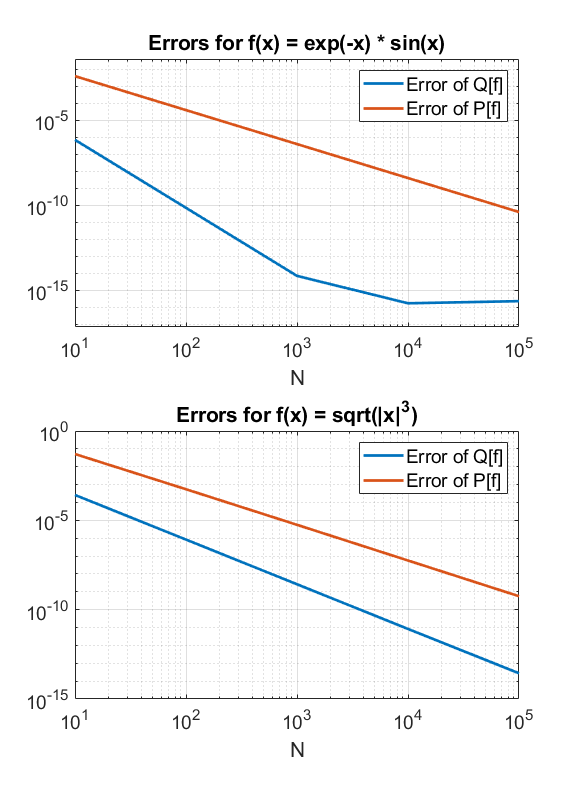
\includegraphics[scale=0.6]{figure.png}
\end{center}

\begin{Verbatim}[frame=single,
   label=\textsc{Matlab} code - analyze.m]
function analyze(f, a, b, I)
   Q = zeros(1, 5);
   P = zeros(1, 5);
   % Calculating the values of the integral calculated
   % using the quadratures Q and P
   for i=1:5
      Q(i) = my_quad(f, a, b, 10^i);
      P(i) = trap(f, a, b, 10^i);
   end

   % Error between real integral and calculated values
   E_Q = abs(Q - I);
   E_P = abs(P - I);

   % Displaying the errors
   fprintf('N = 10^%d; E_Q = %g, E_P = %g\n',...
      [1:5; E_Q; E_P]); 

   % Graphing the errors on a log-log scale
   N = 10.^(1:5);
   loglog(N, E_Q, 'LineWidth', 2);
   hold on;
   loglog(N, E_P, 'LineWidth', 2);

   % Changing the style of the plot
   grid on;
   xlabel('N');
   set(gca, 'FontSize', 14);
   % Setting up the legend
   lgd = legend('Error of Q[f]', 'Error of P[f]');
   set(lgd, 'FontSize', 14);
end
\end{Verbatim}

\begin{Verbatim}[frame=single,
   label=\textsc{Matlab} code - main.m]
% Setting up values for part (d)
I = (1 - exp(-2)*(sin(2) + cos(2)))/2;
f = @(x) exp(-x).*sin(x);
a = 0;
b = 2;
subplot(2, 1, 1);

str = 'exp(-x) * sin(x)';
fprintf('f(x) = %s\n', str);
% Display and graph the errors
analyze(f, a, b, I);
title(sprintf('Errors for f(x) = %s', str));

disp('---');

% Setting up values for part (f)
I = 16/5 * sqrt(2);
f = @(x) sqrt(abs(x).^3);
a = -2;
b = 2;
subplot(2, 1, 2);

str = 'sqrt(|x|^3)';
fprintf('f(x) = %s\n', str);
% Display and graph the errors
analyze(f, a, b, I);
title(sprintf('Errors for f(x) = %s', str));
\end{Verbatim}



\subsection*{(e)}
Because of rounding, there will always be some
error of the order
$I[f]\times u$,
so roughly around $10^{-16}$ in our case. We can see that
for the first integral, the
error between the calculated integral and the real integral of $f$
stops decreasing when it aproaches this value. For this reason,
it makes sense to consider the error calculated for
$N \in \{10, 10^2, 10^3\}$ when calculating the value of $s_1$.

Since we use a log-log scale for the plots, we get that the 
resulting curve can be parametrized by
$y = \log(f(\exp(x)))$.
If we suppose $f$ is $O(x^s)$, then we can approximate $f$ by
$Cx^s$ and so the curve we would get is
$y = \log(C\exp(x)^s) = sx + \log(C)$,
which is just a line of slope $s$. Hence to find $s$, we can just
consider the slope of the line we get on the log-log plot.

We calculate $s_1$ - at $N = 10^1$, we have
$E_Q \approx 6.9\textrm{e}{-7} \approx 10^{-6.2}$, and at
$N = 10^3$, we have
$E_Q \approx 6.8\textrm{e}{-15} \approx 10^{-14.2}$.
So on the log-log plot, we've got an average slope of
$\frac{-14.2 + 6.2}{3 - 1} = -\frac{8}{2} = -4$.
Hence we can conclude $E_Q$ is $O(N^{-4}) = O(h^4)$
and so $s_1 \approx 4$.

Similarly, we calculate $s_2$ - at $N = 10^1$, we have
$E_Q \approx 0.0039 \approx 10^{-2.4}$, and at
$N = 10^5$, we have
$E_Q \approx 3.9\textrm{e}{-11} \approx 10^{-10.4}$.
So on the log-log plot, we've got an average slope of
$\frac{-10.4 + 2.2}{5 - 1} = -\frac{8}{4} = -2$.
Hence we can conclude $E_P$ is $O(N^{-2}) = O(h^2)$
and so $s_2 \approx 2$.
\end{document}
